\chapter{Diskussion}
\textbf{Helene Becker}

% 1. Experiment:
Bei der Kolokalisation von Caspr2 mit VGat und VGlut wurde kein signifikanter Unterschied zwischen den Gruppen festgestellt. Dieses Ergebnis könnte darauf hindeuten, dass Caspr2 nicht bevorzugt an einem bestimmten Synapsentyp vorliegt.
%Fehlerbetrachtung 1.: 
Jedoch ist durch die Ergebnisse keine eindeutige Beantwortung der Forschungsfrage möglich.

Wegen der geringen Datenmenge der SIM-Daten, wurden die WF-Daten statistisch analysiert. Die WF-Daten können als weniger genau angesehen werden. Durch die geringe Auflösung dieser Mikroskopiemethode können kleine Strukturen, wie Synapsen, mikroskopisch und bei der Analyse mit IMARIS nicht voneinander getrennt werden. Es entstehen aus mehreren kleinen Flächen eine große. Deshalb müssen alle WF-Messwerte, die größer sind als 10 $\mu\text{m}^2$, als nicht biologisch realistisch angesehen werden. Daher lässt sich keine abschließende Aussage über das vermehrte Vorhandensein von Caspr2 an hemmenden oder erregenden Synapsen tätigen.
 
 
Zusätzlich funktionierte zwar die Immunfärbung mit VGat und VGlut spezifisch und sauber, doch haben die Primär-AK, die an Caspr2 binden sollten, nicht spezifisch an dieses gebunden. Daher ist keine spezifische Anfärbung von Caspr2 zu Stande gekommen. Mögliche Ursachen dafür sind das Alter (in 2024 bestellt), eine zwischenzeitlich inkorrekte Lagerung oder zu häufiges Einfrieren und Auftauen der Primär-AK. Ersteres ist am wahrscheinlichsten. In weiteren Testfärbungen unserer Fachbetreuerin Josefine Sell am Universitätsklinikum Jena, wurde etwas später die gleiche Färbung mit neu bestellten anti-Caspr2-aAK wiederholt. Ausgetauscht wurden lediglich die Primär-AK für Caspr2. Sie stammen von der gleichen Firma, sind aus der gleichen Spezies gewonnen und lagen in gleicher Konzentration vor. Die Färbung war klarer und die Zellstrukturen in den Dendriten sind deutlich zu erkennen (siehe Abbildung \ref{fig:selltest}), daher ist davon auszugehen, dass die Färbung auf Grund veralteter anti-Caspr2-aAK kaum funktioniert hat.
\clearpage
%\textbf{hier kommt Abbildung 8.1 hin}
\begin{figure}[h] % [h] versucht, das Bild hier zu platzieren (hier), [t] für oben, [b] für unten
	\centering % Zentriert das Bild horizontal
	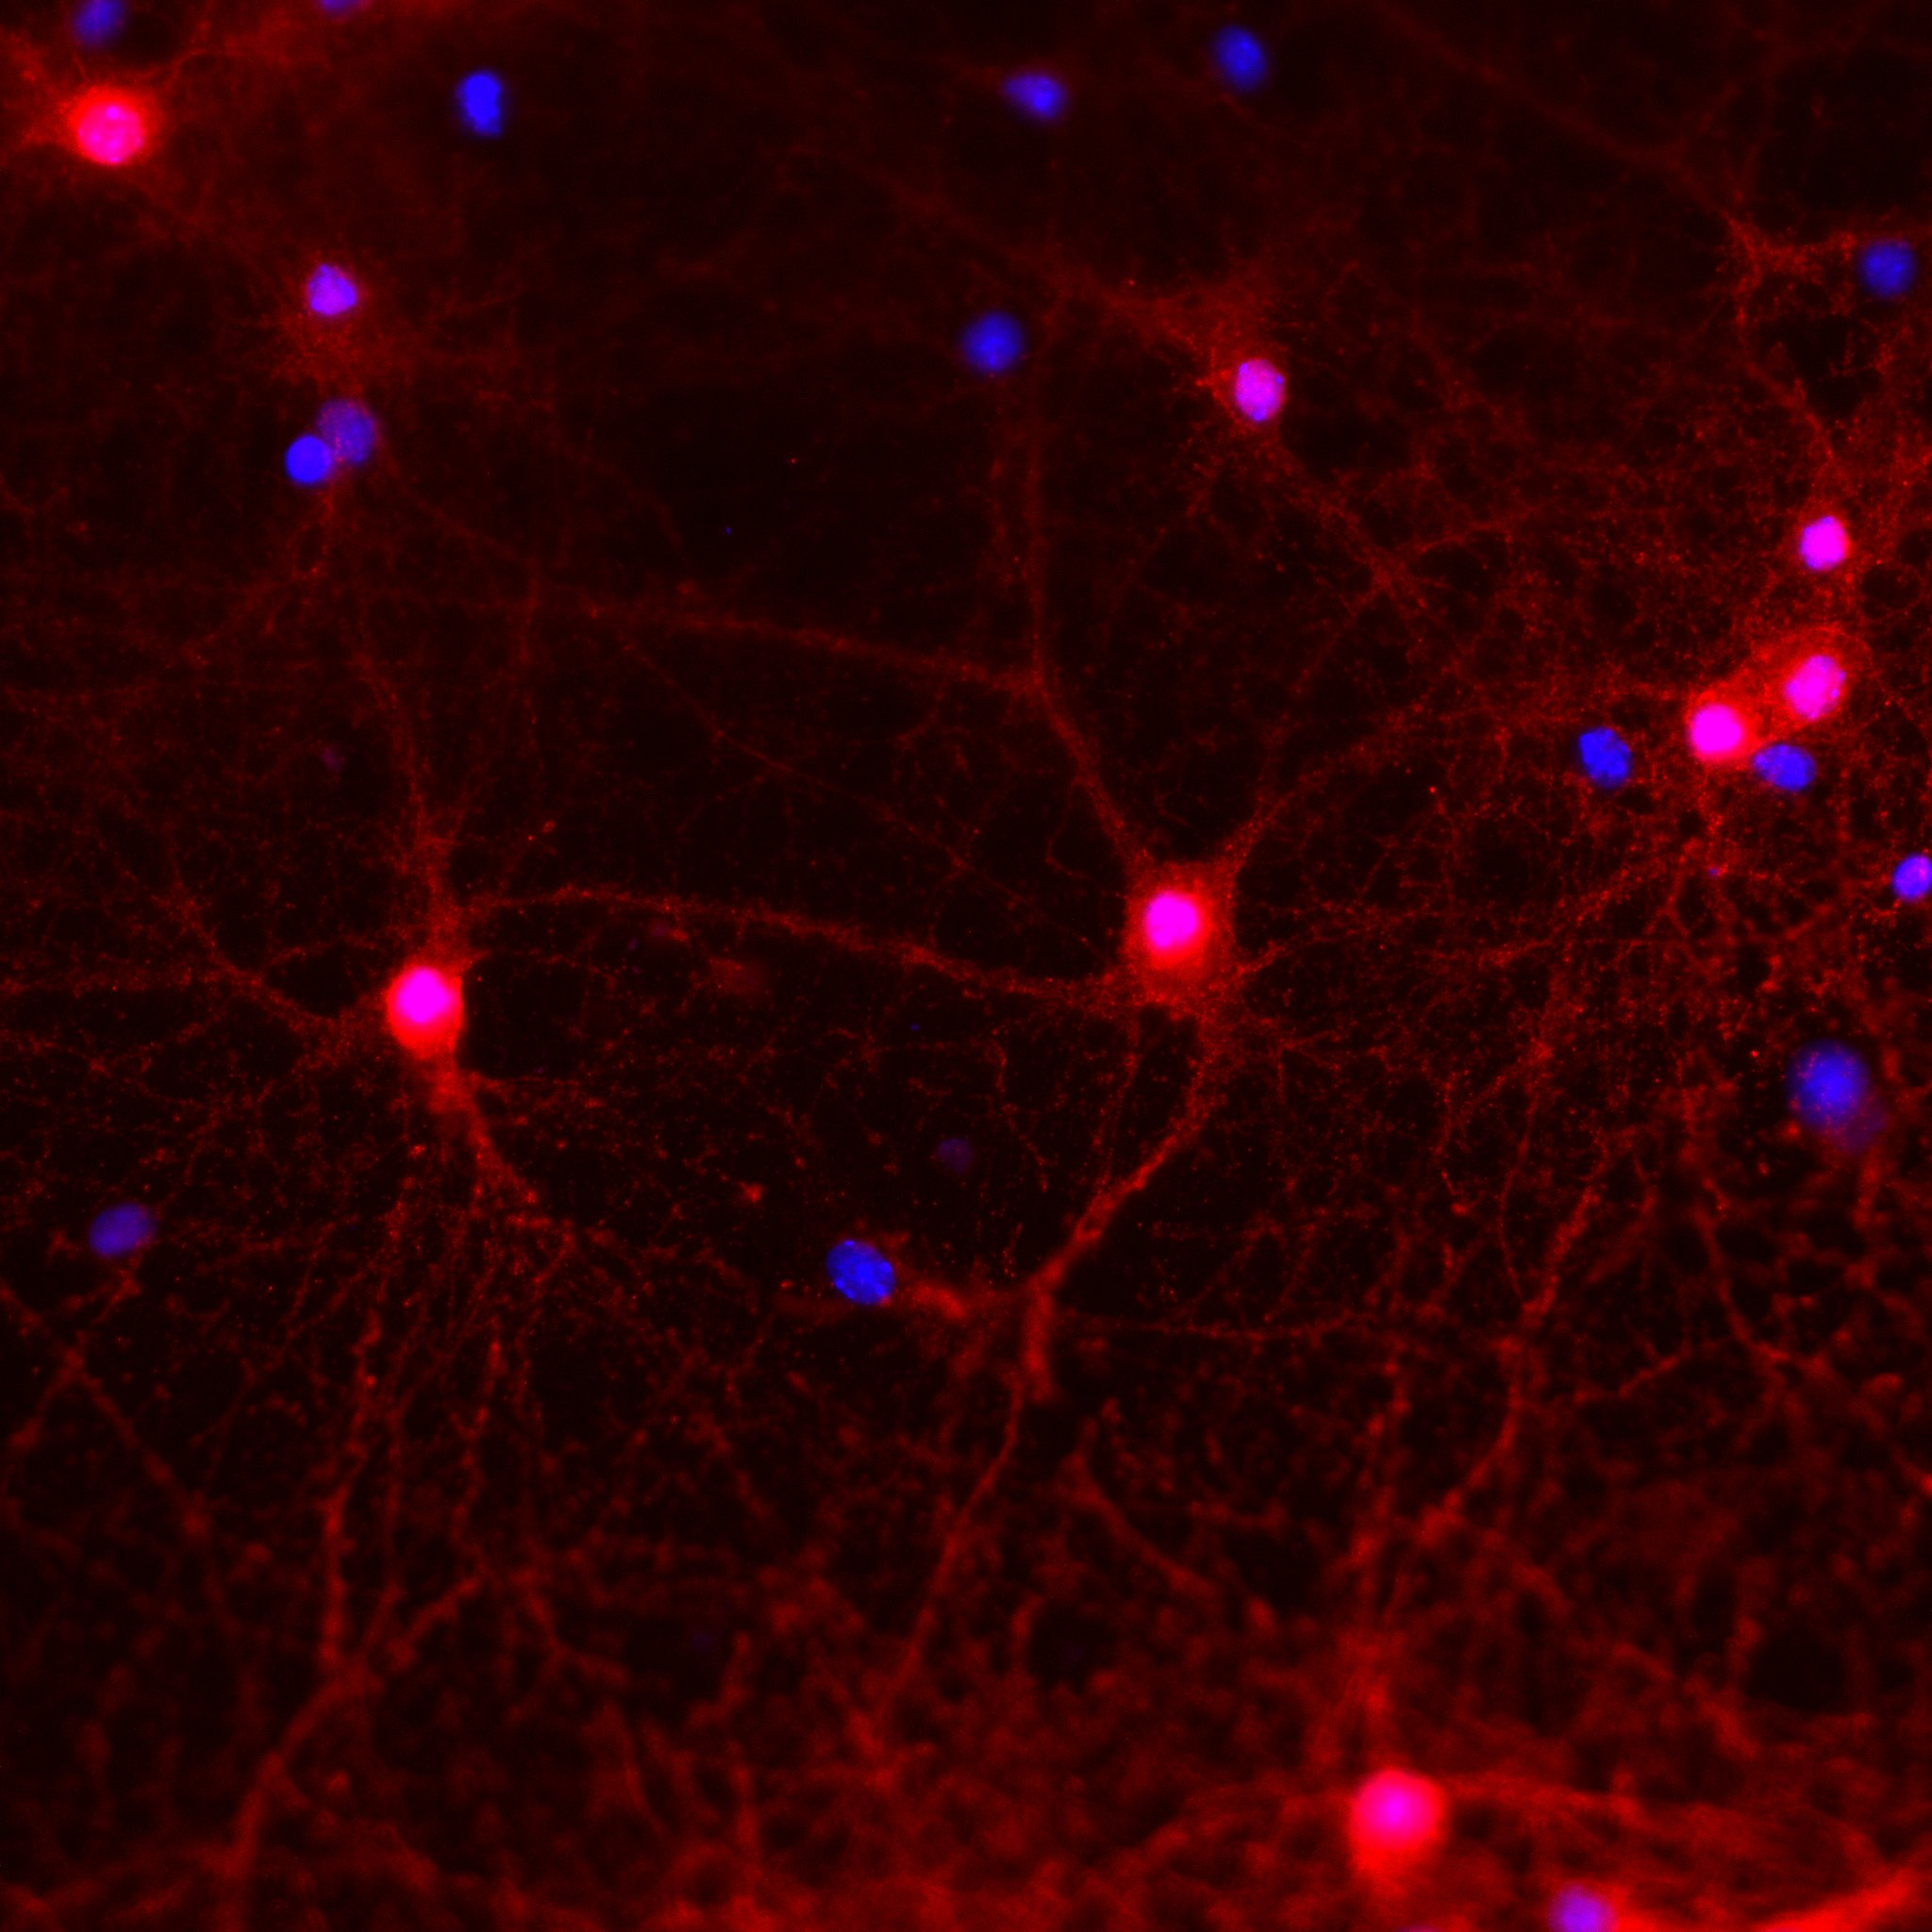
\includegraphics[width=0.91\textwidth]{abbildungen/selltest.png} % Lädt das Bild, skaliert es auf 80% der Textbreite
	\caption{Testfärbung von Josefine Sell mit neuen Primärantikörpern in 40x-Vergrößerung mittels WF. Die fluoreszierenden Strukturen zeigen Caspr2 (rot) und Zellkerne (blau). \parencite{eigenAu8.1}} % Die Bildunterschrift
	\label{fig:selltest} % Ein Label für Querverweise (z.B. "siehe Abbildung \ref{fig:beispielbild}")
\end{figure}
% kolok von caspr2 mit vgat und vglut: kein signifikanter unterschied => deutet darauf hin, dass caspr2 nicht bevorzugt an bestimmten synapsentp vorliegt. jedoch ermöglichen die ergbenisse keine eindeutige beantwortung der forschungsfrage. aufgrund der geringen datenmenge bei SIM wurden die WF daten anaysiert. diese gelten als weniger genau, zusätzlich müssen alle messwerte, dei größer als 10 mikrometer sind, als nicht realistisch angesehen werden. somit lässt sich keine abschließende aussage über das vermehrte vorhandensin von caspr2 an hemmenden oder erregenden synapsen tätigen.
% aktueller forschungsstand zu dieser frage...................
Der aktuelle Forschungsstand zu dieser Frage ist noch gering, dennoch gibt es bereits Ergebnisse, die Hinweise auf die Beantwortung liefern. So konnte in der Studie von Varea et al. aus 2015 das Vorhandensein von Caspr2 an Dendriten, im Soma und an inhibitorischen und exzitatorischen Synapsen festgestellt werden. \footcite[S.~6177]{Varea2015} Des Weiteren wurde eine teilweise Kolokalisation von Caspr2 mit AMPA-Rezeptor-Untereinheiten GluA1 beobachtet. Diese befindet sich auf des postsynaptischen Seite einer exzitatorischen Synapse. Die Kolokalisation mit dem inhibitorischen Marker Gephyrin sei dagegen nicht so hoch gewesen. Daher wird von den Forschenden vermutet, das Caspr2 bezogen auf den Synapsentyp vorrangig an und um exzitatorische Synapsen vorkommt. Weiterhin wären sich unterscheidende Regulationsmechanismen je nach Synapsentyp denkbar. \footcite[S.~6177 f]{Varea2015}

In einer weiteren Studie aus 2015 von Pinatel et al. wurde mittels Immunmarkierung festgestellt, dass 51–68\% der Caspr2-positiven Neuronen auch GAD65-positiv sind. GAD65 kommt ausschließlich an GABAergen Neuronen, also inhibitorischen Neuronen vor. Lediglich 4-8\% der Neuronen waren GAD65-negativ, also exzitatorisch. Die Forschenden kamen zu dem Schluss, dass Caspr2 hauptsächlich an inhibitorischen Neuronen vorliegt. \footcite[S.~4]{Pinatel2015} Bei der Untersuchung der Lokalisation von Caspr2 an Synapsentypen stellten die Forschenden eine Kolokalisation von Caspr2 sowohl mit glutamatergen (exzitatorischen) als auch mit GABAergen (inhibitorischen) präsynaptischen Kontakten fest. Es wird eine besonders hohe Kolokalisation von Caspr2 mit GAD65 beschrieben. So sind 51\% der untersuchten GABAergen Kontakte auch Caspr2-positiv. \footcite[S.~4--6]{Pinatel2015}
Bisherige Studien zeigen unterschiedliche Ergebnisse zu der Fragestellung, an welchem Synapsentyp Caspr2 vorrangig vorliegt.

%\textbf{https://pmc.ncbi.nlm.nih.gov/articles/PMC4434727/pdf/pnas.201423205.pdf (Varea2015)}
% 2. Experiment:
Zwar konnten beim zweiten Teilversuch Ergebnisse aufgenommen werden, allerdings dienen sie nicht der Beantwortung der Forschungsfrage, inwiefern Caspr2-aAK die Kolokalisation zwischen Caspr2 und Contactin2 beeinflusst. 
%Fehlerbetrachung die 2.:
Dies ist auf eine misslungene Kontrollprobe zurückzuführen. Diese sollte ursprünglich dem Vergleich zwischen den mit Caspr2-AK behandelten Neuronen und solchen, die nicht mit den AK behandelt wurden, ermöglichen. Die Forschungsfrage kann aufgrund der fehlerhaften Immunfärbung nicht beantwortet werden. 
Nun wäre lediglich der Vergleich zwischen den AK-Gruppen (also AK gegen die Laminin- bzw. Discoidin-Domäne) möglich.
Die unregelmäßige Verteilung der Kolokalisationsflächen in Abbildung \ref{fig:discSIM} entsteht dadurch, dass bei der Discoidin-Färbung zwei und bei der Laminin-Färbung fünf verschiedene Positionen aufgenommen und ausgewertet wurden. Bei der Discoidin-Färbung war ein sehr großer Teil der Zellen bereits vor dem Färben tot, weshalb wenig sinvolle Positionen aufgenommen werden konnten. In der Laminin-Färbung war dagegen die Zellqualität deutlich besser und die Färbung schien ebenfalls spezifischer zu sein. Dennoch finden sich auch hier tote Zellen (siehe Abbildung \ref{fig:lamininÜB}). Bei der Laminin-Färbung konnten mehr Positionen aufgenommen werden. 
\clearpage
%\textbf{hier kommt Abbildung 8.2 hin}

\begin{figure}[h] % [h] versucht, das Bild hier zu platzieren (hier), [t] für oben, [b] für unten
	\centering % Zentriert das Bild horizontal
	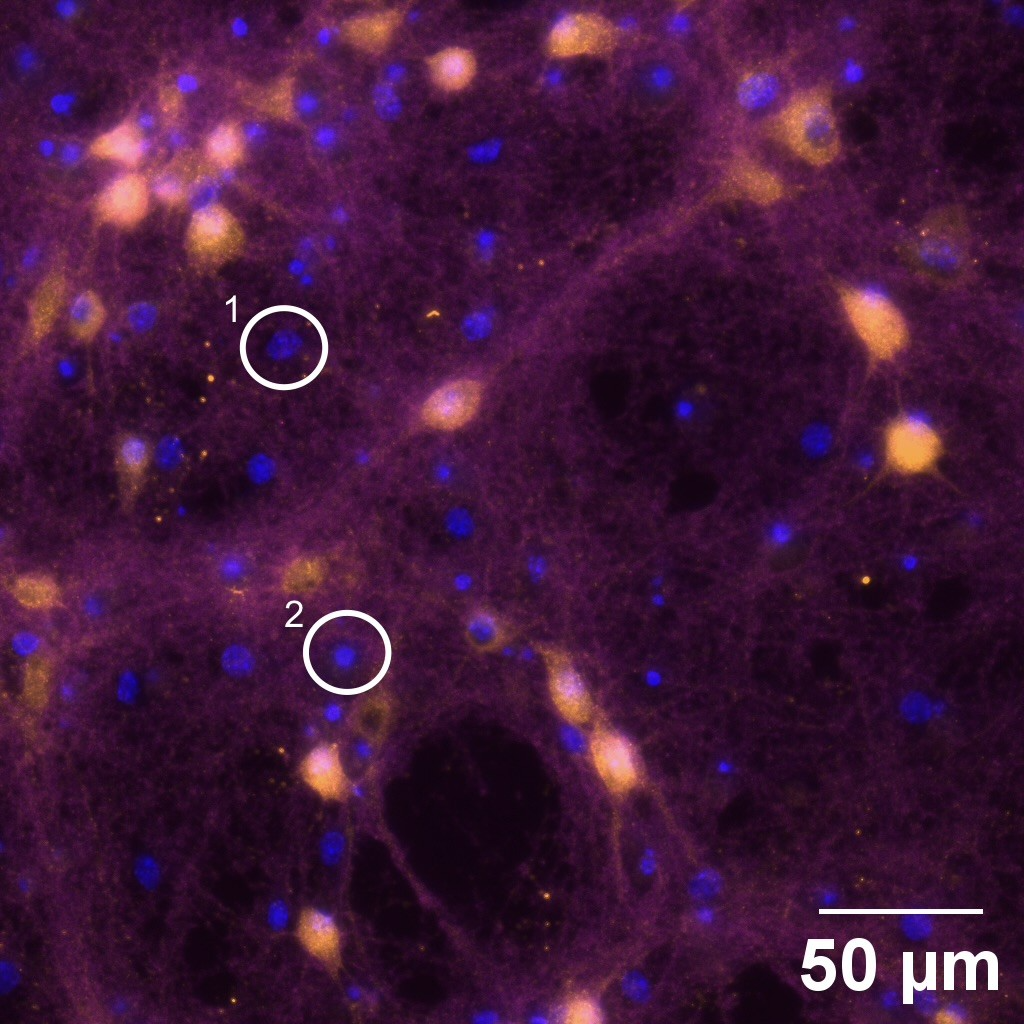
\includegraphics[width=0.91\textwidth]{abbildungen/lamininübersicht.png} % Lädt das Bild, skaliert es auf 80% der Textbreite
	\caption{Übersichtsaufnahme der Laminin-Färbung mittels WF in 20x-Vergrößerung. Die fluoreszierenden Strukturen zeigen Contactin2 (orange), Caspr2 (magenta) und Zellkerne (blau). 1: Zellkern einer lebenden Zelle; 2: Zellkern einer toten Zelle. \parencite{eigenAu8.2}} % Die Bildunterschrift
	\label{fig:lamininÜB} % Ein Label für Querverweise (z.B. "siehe Abbildung \ref{fig:beispielbild}")
\end{figure}
% die ergebisse des 2. teilversuchs dienen nicht der beantwortung der Forschungsfrage, inwiefern Caspr2-aAK die Kolok zw Caspr2 und Contactin2 beeinflussen. aufgrund einer misslungenen kontrollprobe ist der vergelcih zwischen anti-Caspr2-AK behandelten neuronen und solchen, die nicht mit anti-Caspr2-AK behandelt wurden nun nicht möglich. lediglich der verglich zw den ak gruppen gegen die Laminin bzw disoidin domäne wäre möglich. die forschungsfrage kann aufgrund der fehlerhaften immunfärbung daher nicht beantwortet werden.
% aktueller Froschungsstand Im gegensatz zur ersten Untersuchung liegen für diese Fragestellung bereits einige Forschungen und Literatur vor..............
Im Gegensatz zur ersten Untersuchung scheinen  zur Beantwortung der Frage, welchen Einfluss die aAK auf die Proteininteraktion zwischen Caspr2 und Contactin2 haben, bereits mehr Studien vorzuliegen.
2018 wurde von Patterson et al. gezeigt, dass durch die Bindung von Caspr2-aAK an Caspr2 die Interaktion zwischen Caspr2 und Contactin2 gehemmt wird. \footcite[S.~6, 8]{Patterson2018} 
Bezüglich der zweiten Fragestellung finden sich verschiedene Hypothesen und Ergebnisse. Patterson et al. konnten eine gestörte Interaktion von Caspr2 und Contactin2 zeigen. Eine andere Studie von Saint-Martin et al. aus 2019 zeigt, dass anti-Caspr2-aAK zwar keine Auswirkung auf die Internalisierung (zelluläre Aufnahme) von Caspr2 haben, aber die Oberflächenverteilung, sowie die Interaktion von Caspr2 mit TAG1 (= Contactin2) beeinflussen. Die AK führen der Studie nach zu einer erhöhten Oberflächenexpression und Clusterbildung (gesteuerte Zusammenlagerung von Proteinmolekülen zu größeren Strukturen) von Caspr2. \footcite[S.~8]{SaintMartin2019} Die Beeinträchtigung der Bindung von Caspr2 zu TAG1/Contactin2 ist nicht so stark ausgefallen wie in der Studie von Patterson et al.. Solche Unterschiede sind auf die verschiedenen Methoden zurück zuführen. So nutzten Patterson et al. ein zellfreies Bindungsassay während Saint-Martin et al. ein zelluläres Modell nutzen. Im zellfreien Bindungsassay werden die Proteine direkt miteinander inkubiert, während in einem zellulären Modell zusätzliche Faktoren, wie bspw. die räumliche Anordnung der Proteine oder ihre Oberflächenexpression, die Messungen beeinflussen und die Bindung abschwächen. \footcite{SynapsebyPatsnap2025} 
\textbf{https://synapse.patsnap.com/article/what-is-the-difference-between-cell-free-and-cell-based-expression-systems (SynapsebyPatsnap2025)}
In einer anderen Studie wird ebenfalls von einer Beeinträchtigung der Interaktion von Caspr2 mit Contactin2 gesprochen. \footcite[S.~11, 15 f]{VanHoof2024}

In weiterführenden Studien konnte ebenfalls gezeigt werden, dass anti-Caspr2-aAK einen Einfluss auf die räumliche Organisation des VGKC-Komplexes haben. \footcite[S.~10]{Habib2025} Dieser Komplex ist bereits in Kapitel 3 Abbildung \ref{fig:cmyelin} dargestellt. Es handelt sich um einen Proteinkomplex von spannungsabhängigen Kaliumkanälen, deren Bestandteil auch Caspr2 ist. Bei Patienten, die symptomatische Schmerzen aufwiesen, führte eine Bindung von anti-Caspr2-aAK zu einem signifikanten Anstieg des Abstandes zwischen dem Kv1.2-Kanal und Caspr2. Dies deute darauf hin, dass der Proteinkomplex (das schließt auch Contactin2 ein) seine strukturelle Widerstandsfähigkeit aufgrund der AK-Bindung verliert. Zudem zeigten die Serumproben dieser Patienten bei der Untersuchung der neuronalen Erregbarkeit eine verstärke Aktivität, sowie eine geminderte Aktivität der Kaliumionen-Kanäle. Daher könne es sein, dass die Veränderung der neuronalen Aktivität direkt mit der Bindung der Caspr2-aAK zusammenhängt und somit auch die Funktionalität des VGKC-Komplexes. \footcite[S.~10]{Habib2025} Ein Unterschied zwischen den AK Gruppen, die an die Laminin- oder Discoidin-Domäne binden wurde nicht untersucht. Allerdings scheint die IgG-Subklasse eine Rolle bei der Ausbildung von Symptomen, wie neuropathischen Schmerz, der untersuchten Patienten zu spielen. \footcite[S.~10 f]{Habib2025} Obwohl die Discoidin-Domäne für die Bindung der anti-Caspr2-aAK von Bedeutung ist, \footcite[S.~11]{VanHoof2024} scheint sie für die Caspr2–Contactin-2-Interaktion selbst nicht erforderlich zu sein. Die Untersuchungen von Saint-Martin et al. weisen eher darauf hin, dass insbesondere die Laminin-G1-Domäne von Caspr2 wesentlich für die Interaktion von Caspr2 mit TAG1/Contactin2 sind. So stören anti-Caspr2-aAK die Interaktion hauptsächlich durch die Laminin-G1-Domäne. \footcite[S.~9]{SaintMartin2019} 
In der Studie von Oliveira et al. aus 2026 konnte auch an menschlichen neuronalen Organoiden (= organähnliche 3D-Strukturen, die im Labor aus Stammzellen gezüchtet werden, ahmen Struktur sowie Funktion echter Organe nach) beobachtet werden, dass nach einer Behandlung dieser mit anti-Caspr2-aAK die Feuerrate der AP signifikant höher ist als ohne die Behandlung mit anti-Caspr2-aAK. Somit konnte gezeigt werden, dass anti-Caspr2-aAK sowohl die neuronale Funktionalität, als auch die neuronale Entwicklung beeinflussen kann. \footcite[S.~8 f]{Oliveira2026} Ein Unterschied der Methode von Oliveira et al. zu der in dieser Arbeit ist besonders relevant. Oliveira et al. untersuchte die Embryonalentwicklung und nicht die Autoimmunreaktion in adulten Organismen. Die Studie zeigt die funktionellen Folgen einer anti-Caspr2-aAK-Bindung, bezieht sich allerdings nicht direkt auf die Interaktion zwischen Caspr2 und Contactin2. Des Weiteren sei angemerkt, dass die Fragestellung sowie die Durchführung unserer Untersuchung der Veröffentlichung dieser Studie voraus ging.


%\textbf{https://pub.dzne.de/record/279357/files/DZNE-2025-00734.pdf?subformat=pdfa (Habib2025)}
%
%\textbf{https://pmc.ncbi.nlm.nih.gov/articles/PMC5876120/pdf/nihms930925.pdf  (Patterson2018) ich glaube, wir haben diese Quelle schoneinmal verwendet}
%
%\textbf{https://pmc.ncbi.nlm.nih.gov/articles/PMC12926859/pdf/JNC-170-0.pdf (Oliveira2026)}
%
%\textbf{https://pmc.ncbi.nlm.nih.gov/articles/PMC7618075/pdf/EMS208257.pdf (VanHoof2024)}


% allgemeine Fehlerbetrachtung: 
% es wurde... untersucht, im verlauf zeigte sich, dass die messergebnisse nicht/ nur eingeschränkt interprtiert werden können. daher ist im folgenden zu betrachten, welche Faktoren zu den Einschränkungen der UNtersucheungen beigetragen haben. 
% 1. zwar haben die immunfärbungen mit VGat und VGlut spezifisch und sauber funktioniert, doch die primär Ak zur Färbung des Caspr2 haben nicht an das protein gebunden. dadurch ist keine spezifische anfärbung des Caspr2 zu stande gekommen. Mögliche Ursachen sind, dann die AK bereits zu alt geworden waren (2024 bestellt). eine weitere Möglichkeit ist, dass sie kurzzeitig falsch gelagert oder zu häufig eingefroren und wieder aufgetaut wurden, 
% \textbf{um sie für verschiedene andere versuche zu nutzen?}. 
% in weiteren testfärbungen des Uiveritätsklinikums Jena von der forschungsgruppe ...... wurde die gleiche färbung mit neuen primär AK, der gleichen Firma, Spezies (@sheep???) und Verdünnung, und gleichen sekundär AK durchgeführt. diese lieferten klarere Färbungen. (siehe bild von josefine) es ist davon auszugehen, dass die Färbung aufgrund veralteter anti-Caspr2-AK nicht funktioniert hat.

% - für Discoidin-AK hatten wir nur 2 Positionen aufgenommen (hier waren ein Großteil der Zellen schon vor dem Färben tot und kaputt und wir konnten nur wenig brauchbare Positionen finden)
% - Für Laminin1-AK haben wir insgesamt 5 Positionen von 2 verschiedenen Deckgläsern aufgenommen (die Zellqualität war besser und die Färbung sah auch recht gut aus. Deswegen gibt es hier viele Stellen, die kolokalisiert waren).
% im 2. versuch, wurde mit liveinkubation gearbeitet. dabei gab es wahrscheinlich keine Reaktivität zwischen den @sheep-AK und den Maus-neuronen


Es zeigt sich, dass die Messergebnisse unsere Versuche nur eingeschränkt interpretiert werden können.





